\documentclass[12pt]{article} 

\usepackage{amsmath, amsfonts, amssymb, graphicx}

\title{results so far}
% \author{Thomas Johnson}

\begin{document}
\maketitle

Used the Google stock back to November 2010 up until now. Used the data from 2010 until January 1st 2015 to generate the elements of the transition matrix. Then tried to estimate from January 1st to today using the models.

Here's what the stock looks like:

\begin{figure}[hb]
\caption{The blue part is used to fill up the transition matrices, and then tried to estimate the black part.}
\centering
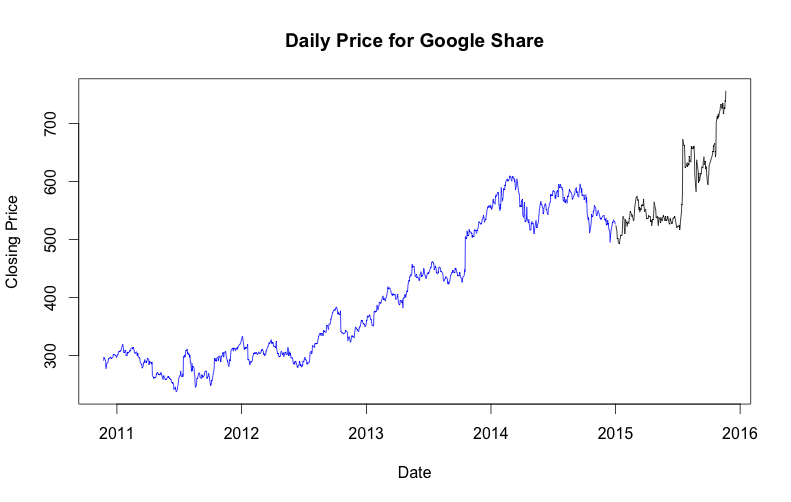
\includegraphics[width=5.5in]{general_trend.png}
\end{figure}

\newpage
Model 1 has the states:
\begin{enumerate}
\item increase from the day before ($A$)
\item decrease from the day before ($B$)
\end{enumerate}
This is what the transition matrix came out to be
$$
\bordermatrix{~ & A & B \cr
                  A & 0.5205993 & 0.4794007 \cr
                  B & 0.5130785 & 0.4869215 \cr}
$$

Here are some trials for estimating what happens in 2015 using this model (simulation uses random numbers so comes out different every time)

\begin{figure}[hb]
%\caption{}
\centering
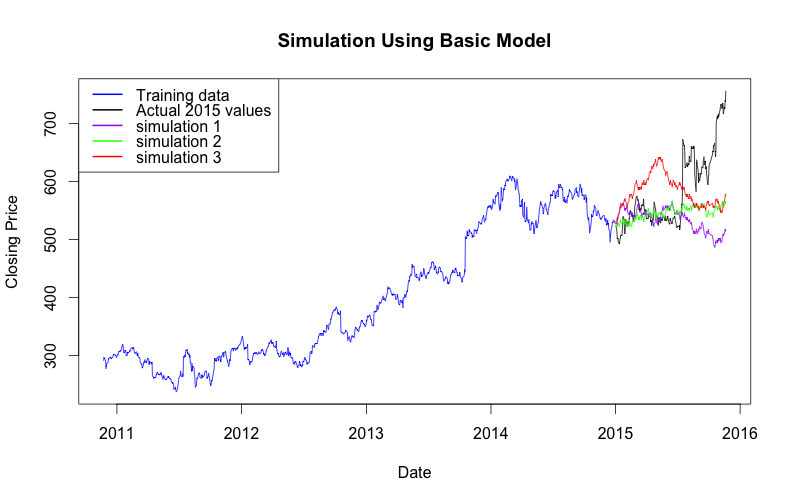
\includegraphics[width=5.5in]{basic_model.png}
\end{figure}

\newpage
Model 2 has the states:
\begin{enumerate}
\item large increase from the day before ($A$)
\item small increase from the day before ($B$)
\item small decrease from the day before ($C$)
\item large decrease from the day before ($D$)
\end{enumerate}
This is what the transition matrix came out to be
$$
\bordermatrix{~ & A & B & C & D \cr
                  A & 0.2238095 & 0.3190476 & 0.2952381 & 0.1619048 \cr
		 B & 0.1882716 & 0.3179012 & 0.3487654 & 0.1450617 \cr
	         C & 0.1932515 & 0.3006135 & 0.3251534 & 0.1809816 \cr
		 D & 0.2222222 & 0.3274854 & 0.2631579 & 0.1871345 \cr}
$$

Here are some trials for estimating what happens in 2015 using this model

\begin{figure}[hb]
%\caption{}
\centering
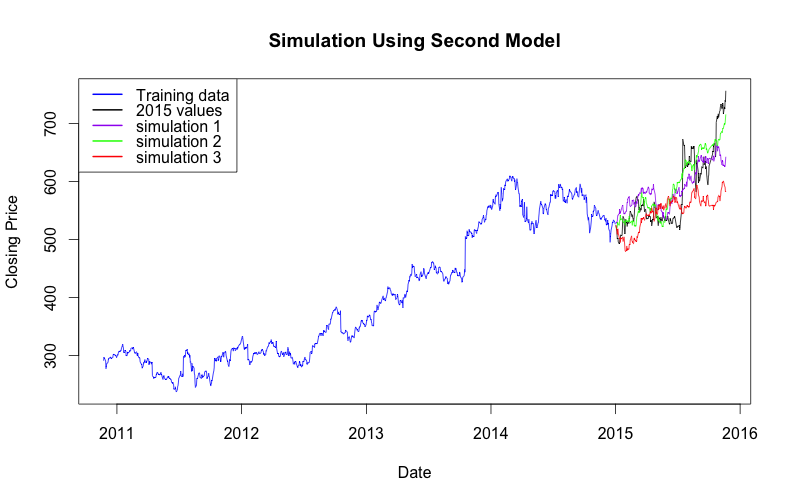
\includegraphics[width=5.5in]{model_2.png}
\end{figure}

\end{document}

